\chapter{Part 1} % (fold)
\label{cha:part_1}

\centering
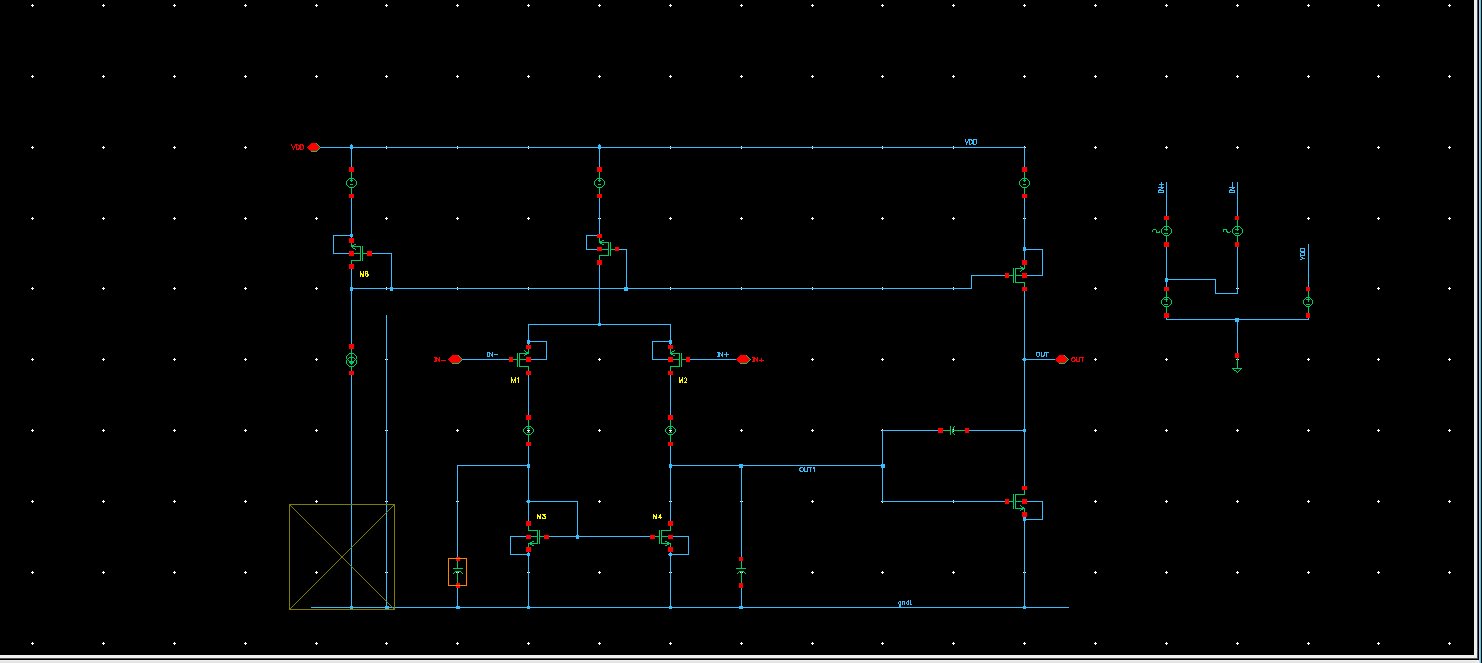
\includegraphics[width=1\textwidth]{Capitoli/whole.png}
\raggedright


\section{Gain, Bandwith and Stability} % (fold)
\label{sec:gain_and_bandwith}

\subsection{Gain} % (fold)
\label{subsec:gain}



As first step starting from the gain requirements we choose the lenght of transistors $M_1,M_2,M_3,M_4,M_6,M_7.$

Splitting the gain in half beetween the 2 stages we get\footnote{The evaluation of the second stage's gain has been done exactly in the same way}:

\begin{equation}
	G_{1^{st} stage} = 100 = \frac{2V_AL_1L_3}{V_{ov_1}L_{min}(L_1+L_3)}
\end{equation}


In this first step we decided to keep $L_1=L_2=L_3=L_4$ and $L_6=L_7$.

Respecting the constraint of $V_{ov_x} > 200mv$ we choose:

\begin{itemize}
	\item $V_{ov_1}=V_{ov_2}= 0.2V$ in order to keep the $g_m$ as high as possible in order to respect the bandwith specification\footnote{This will be also good for phase margin}.
	\item $V_{ov_3}=V_{ov_4}= 0.3V$ in this way we will have $g_{m3}=g_{m4}<g_{m1}=g_{m2}=$, squeezing the input referred noise.
	\item $V_{ov_5}= 0.4V$ to minimize the area\footnote{Accepting some losses in terms of CMRR}.
	\item $V_{ov_6}=V_{ov_7}= 0.2V$ in order to keep o good output voltage swing. 
\end{itemize}

% section gain (end)

\subsection{Bandwidth} % (fold)
\label{subsec:bandwidth}



Then starting from the bandwith and the phase margin specifications we tune the transconductance of the input pair and the value of the compensation capacitance, going through this calculation:

\begin{equation}
	GBWP=40MHz=\frac{g_{m1}}{2 \pi C_c}
\end{equation}
Assuming for this step $C_c = 1pF$
Then we will check if the choosen values keep us in the stability contraint.



\centering
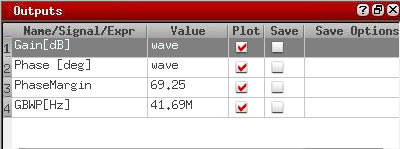
\includegraphics[width=0.5\textwidth]{Capitoli/gainprimo.png}
\raggedright

% section bandwidth (end)

\subsection{Phase Margin} % (fold)
\label{subsec:phase_margin}

\begin{equation}
	C_c> \frac{g_{m1}}{g_{m6}}(C_1+C_L)
\end{equation}

During all the design we are going to assume a load capacitance of 1pF.
At this moment the M6's were not yet fixed , but for this calcultaion we assume $C_1+C_L=2pF$\footnote{We will check at the end that this assumption results confirmed.}

\begin{equation}
	\phi_m=180- actg(\frac {GBWP} {f_o} )-acrtg(\frac { g_{m1} }{ g_{m6}})-arctg(\frac{g_{m1}} {C_c}\frac{C_L+C_1}{g_{m6}})=60 
\end{equation}

From this equation we get $g_{m6} = 2mS $ which is quite high , but using this stage\footnote{Which gives a positive zero.} we have deal with some trade-offs.

From the transconductance of M6 we can find the current flowing in the second stage:
\begin{equation}
  I_6=I_7= \frac{g_{m6}V_{ov_6}}{2}
\end{equation}

and the form factors:

\begin{itemize}
    \item $(\frac{W}{L})_6=200=\frac{200 \mu m}{1 \mu m}$
 
    \item $(\frac{W}{L})_7=100=\frac{100 \mu m}{1 \mu m}$
    
  \end{itemize}  

Now that we know as $L_6$ as $w_6$ we can verify the real value of $C_1$ which result to be:

\begin{equation}
  C_1 = C_{ox} \gamma W_6 L_6 = 0.66pF
\end{equation}

which confirm our hypotesys made in the step of the compensation capacitance sizing\footnote{As the real value is lower than the one used for calculation the performances are going to be improved}.

\centering
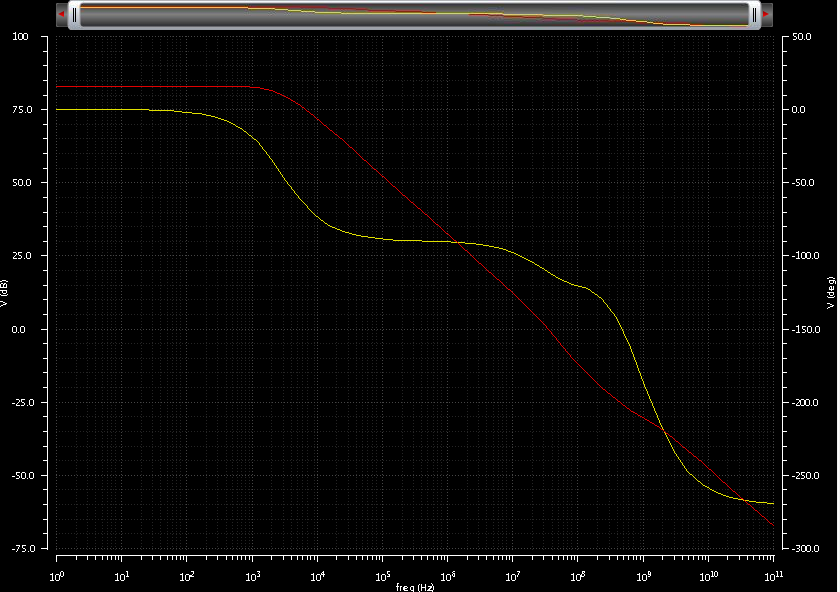
\includegraphics[width=1\textwidth]{Capitoli/gainph1.png}
\raggedright


% section phase_margin (end)

% section gain_and_bandwith (end)

\section{Noise} % (fold)
\label{sec:noise}


\subsection{White Noise} % (fold)
\label{ssub:white_noise}


The input referred noise with this sizing results to be:

\begin{equation}
  S_v^n= \frac{8KT\gamma}{g_{m1}}(1+\frac{g_ {m3}}{g_{m1}}) = (11.51 \frac{nV}{\sqrt{Hz}})^2
\end{equation}

In order to reduce $g_{m3,4}$ and to get our target we decide to increase $V_{ov_4}$ to $0.4V$
% subsubsection white_noise (end)

\centering
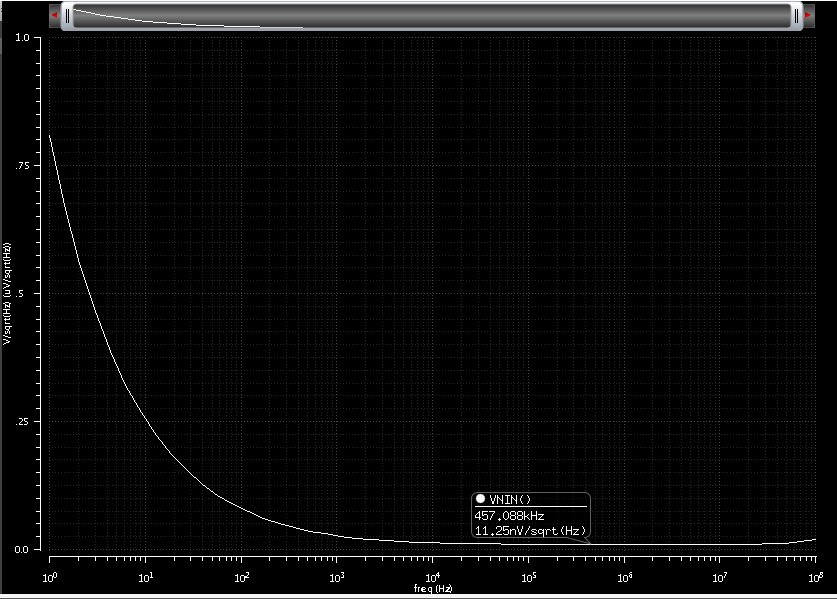
\includegraphics[width=1\textwidth]{Capitoli/wn1st.png}
\raggedright



\subsection{Noise Corner Frequency} % (fold)
\label{ssub:noise_corner_frequency}

The NCF results to be in order of $100KHz$ so we decided to increse $(WL)_{3,4}$ of a factor 6,5 in order to have the NCF below 10KHz.


\centering
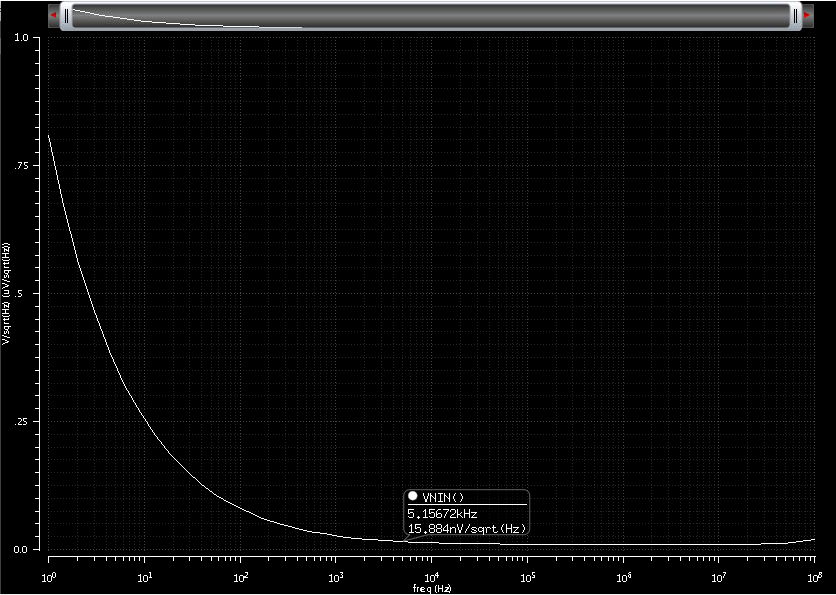
\includegraphics[width=1\textwidth]{Capitoli/ncf1.png}
\raggedright

% subsubsection noise_corner_frequency (end)

% section noise (end)

\section{Results} % (fold)
\label{sec:results}


\begin{equation}
  E_n^2=( 11.51 \frac {nV} { \sqrt{HZ}})^2
\end{equation}

\begin{equation}
  \phi_m=69.25
\end{equation}

\begin{equation}
  GBWP=41.69MHz
\end{equation}

\begin{equation}
  Gain=83.55dB
\end{equation}
% section results (end)

\begin{equation}
  Current \ \ Consumption = 813.5 \mu A
\end{equation}


\begin{table}[]
\centering
\caption{PART 1 SIZING}
\label{my-label}
\begin{tabular}{|l|l|l|l|l|l|l|}
\hline
      & W      & L      & I      & V\_d   & V\_s & V\_g   \\ \hline
M1 M2 & 25u    & 1u     & 26.62u & 0.994V & 2.3V & 1.5V   \\ \hline
M3 M4 & 16.8u  & 4.965u & 26.62u & 0.994V & 0V   & 0.994V \\ \hline
M5    & 4.375u & 0.35u  & 53.24u & 2.3V   & 3V   & 2.007V \\ \hline
M6    & 150u   & 1.5u   & 815u   & 1.408V & 0V   & 0.994V \\ \hline
M7    & 300u   & 1.5u   & 815u   & 1.480V & 3V   & 2.027V \\ \hline
M8    & 0.35u  & 0.35u  & 4u     & 2.007V & 3V   & 2.007V \\ \hline
\end{tabular}
\end{table}


\subsubsection{Sources} % (fold)
\label{ssub:sources}


On this Github repo you can find the Cadence cchematics of both circuits presented compressed in the file : Project_Zero_Merged_V6.gz.



% subsubsection sources (end)
% chapter part_1 (end)